\documentclass{article}

\usepackage[left=2cm,right=2cm, top=2cm, bottom = 2cm]{geometry}
\usepackage{amsfonts}
%%%\usepackage{array}

\usepackage{amsmath}
\usepackage{xcolor}

\usepackage{tikz}
\usepackage{subfigure}

\pagestyle{empty}

\setlength{\tabcolsep}{15pt}
%%%\renewcommand{\arraystretch}{2.5}

%%%\makeatletter
%%%\newcommand{\thickhline}{%
%%%    \noalign {\ifnum 0=`}\fi \hrule height 2pt
%%%    \futurelet \reserved@a \@xhline
%%%}
%%%\newcolumntype{!}{@{\hskip\tabcolsep\vrule width 2pt\hskip\tabcolsep}}
%%%\makeatother

\newcommand{\deriv}[2]{\frac{\mathrm{d}#1}{\mathrm{d}#2}}
\newcommand{\diff}{\;\mathrm{d}}


\usepackage{pgfplots}

\pgfplotsset{compat=1.10}
\usepgfplotslibrary{fillbetween}
\usetikzlibrary{patterns}


\begin{document}

\title{Signed Areas}
\date{}

\maketitle
\thispagestyle{empty}

\Large

\textbf{\underline{Objective: To understand the notion of an area with a sign.}}






\vspace{5mm}



\textbf{Recap: Antiderivatives and the Fundamental Theorem of Calculus:}\bigskip


\begin{enumerate}
	\item Find an antiderivative of $3x^{-4}$.
	\item
		\begin{enumerate}
			\item Give a general expression for
				\[\int x^{-n}\diff x,\]
				where $n\neq -1$.
			\item What is
				\[\int x^{-1}\diff x?\]
		\end{enumerate}
	\item Evaluate
		\[\int_0^\frac{\pi}{2} \sin(x)\diff x.\]
\end{enumerate}






\clearpage


\textbf{Warm-up: Signed Areas:}\bigskip



\begin{enumerate}
	\item Evaluate:
		\begin{enumerate}
			\item
				\[\int_0^\pi \cos(t)\diff t\]
			\item
				\[\int_0^\frac{\pi}{2}\cos(t)\diff t\]
			\item
				\[\int_\frac{\pi}{2}^\pi \cos(t)\diff t\]
		\end{enumerate}
	\item Sketch the graph of $\cos(t)$ (if you haven't already). What is the area between the curve $x=\cos(t)$ and the $t$-axis?
\end{enumerate}



\clearpage


\textbf{Theory: Signed Areas:}

\bigskip


When we first introduced integration, we said that it gives the area under a curve. This isn't quite true: an area is always positive, but an integral can be negative. If the function being integrated is above the horizontal axis, then the integral gives the area; if it is below the axis, then the integral gives \textit{minus} the area. If the function crosses the axis within the domain of integration, then the integral gives the difference between the areas.\medskip

\begin{center}
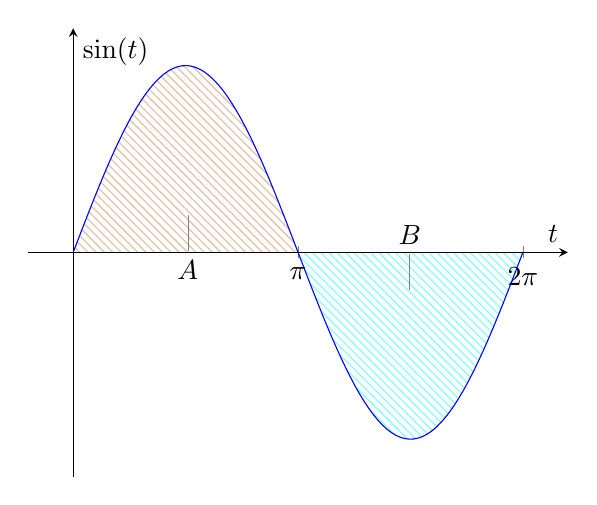
\begin{tikzpicture}
	\begin{axis}[axis lines=middle,
		            xlabel=$t$,
		            ylabel=$\sin(t)$,
	           	 enlargelimits,
           		 ytick=\empty,
		            xtick={3.14,6.28},
           	 	xticklabels={$\pi$, $2\pi$}
           	 ]
		
		\addplot[name path=F,blue,domain={0:6.28},samples=100] {sin(x*180/3.14)};

		\addplot[name path=G,domain={0:6.28}] {0};

		\addplot[pattern=north west lines, pattern color=brown!50]fill between[of=F and G, soft clip={domain=0:3.14}];
		\node[coordinate,pin=270:{$A$}] at (axis cs:1.6,0.2){};
		
		\addplot[pattern=north west lines, pattern color=cyan!50]fill between[of=F and G, soft clip={domain=3.14:6.28}];
		\node[coordinate,pin=90:{$B$}] at (axis cs:4.7,-0.2){};
	\end{axis}
\end{tikzpicture}
\end{center}

In the above diagram, the area $A$ is the integral of $\sin(t)$ from $0$ to $\pi$, while the area $B$ is \textit{minus} the integral of $\sin(t)$ from $\pi$ to $2\pi$:
\begin{align*}
	A&=\int_0^\pi \sin(t)\diff t = 2\\
	B&=-\int_\pi^{2\pi}\sin(t)\diff t = 2\\
\end{align*}
The total area enclosed between the curve and the $t$-axis is therefore $A+B=4$, whereas the integral of $\sin(t)$ from $0$ to $2\pi$ is $A-B=0$:
\[\int_0^{2\pi}\sin(t)\diff t=0.\]

This is not always a bad thing:\medskip


Suppose a ball is thrown in the air from $y=10\mathrm{m}$ at time $0$, with velocity given by $y'(t)=(1-t^2)\mathrm{ms^{-1}}$. Find the position after 2s, and the total distance travelled in those 2s.

\clearpage


\textbf{Theory: Reversing the Limits of Integration:}\bigskip


There is another way that an integral can give a negative answer---even when the integrand (the function being integrated) is positive! This is to do with the order of the limits of integration:\medskip

Working directly from the definition of the integral, evaluate
\[\int_4^0 x\diff x.\]
Compare both with the area enclosed by the curve, and with the answer gained from the antiderivative method of evaluating integrals.


\vfill


Evaluate
\[\int_5^{719} x^3e^{\sin\left(x^{-3}\right)}\diff x + \int_{719}^5  x^3e^{\sin\left(x^{-3}\right)}\diff x.\]

\vfill


\clearpage


















\textbf{Practice:}\bigskip





\begin{enumerate}
	\item Find the total area between the curve $y=3e^x-7$ and the $x$-axis for $0\leq x\leq 2$. How much of this area is above the $x$-axis, and how much is below?
	\item The current flowing onto one plate of a capacitor is given by $I(t)=200\sin(100\pi t)\mathrm{mA}$. Initially the capacitor has $50\mathrm{mC}$ of charge on it. Find the charge on the capacitor at $t=30\mathrm{ms}$. What is the maximum charge on the capacitor in the first $30\mathrm{ms}$, and at what time does it occur?
	\item Find the total area between the curves $y=x$ and $y=x^2$ between $x=0$ and $x=2$. Hint: draw a diagram.
\end{enumerate}








\clearpage













{\bf Key Points to Remember:}

\vspace{5mm}

\begin{enumerate}
	\item A definite integral counts areas above the horizontal axis as positive and below the axis as negative; it can therefore give a negative answer or 0 because of positive and negative areas cancelling each other out.
	\item To find the total area between a curve and the horizontal axis, split the domain of integration into sections over which the curve is always above or always below the axis, integrate over each interval separately, and add up the absolute values of the answers.
	\item When looking for the change in a quantity between two times, we integrate the derivative directly---negative areas cancelling out positive amounts to decreases in the quantity undoing increases. For instance, the distance from a moving particle's start position to end position is the integral of the velocity.
	\item When looking for the total amount of change in a quantity---regardless of which way the change is---we find the total area, so split the domain of integration into positive and negative parts and add up the absolute values. For instance, the total distance travelled by a particle is the total area enclosed by its velocity-time curve.
	\item To find the area between two curves, we can integrate each separately and subtract.
	\item Reversing the order of the limits of an integral has the same effect as multiplying the integral by $-1$.
\end{enumerate}









\end{document}